\documentclass{beamer}
%\usetheme{Malmoe}
\usetheme{metropolis}

\usepackage[utf8]{inputenc}
\usepackage{amsmath}
\usepackage{amsfonts}
\usepackage{amssymb}
\usepackage{graphicx}
\graphicspath{{./src/}}
%\author{}
%\title{}
%\setbeamercovered{transparent} 
%\setbeamertemplate{navigation symbols}{} 
%\logo{} 
%\institute{} 
%\date{} 
%\subject{} 
\title{Luplink : Link Budget Calculation UI}
\subtitle{}
\author{Julien Prissimitzis\\
\bigskip
Supervisor: Thibault Gateau}
\institute{DCAS ISAE-Supaero}

\date{\today}
\setbeamercolor{block title}{use=structure, bg=white}
%\setbeamercolor{block body}{use=structure,fg=black,bg=blue!10!white}
%\setbeamertemplate{blocks}[rounded][shadow=false]
\setbeamercolor{background canvas}{bg=white}
\begin{document}

%\begin{frame}
%\titlepage
%\end{frame}

%\begin{frame}
%\tableofcontents
%\end{frame}

\begin{frame}
	\titlepage
\end{frame}

\section{Link Budget \& Context}

\begin{frame}
	\frametitle{Link Budget \& Context}
%\textbf{Goal:} Communication with a satellite

%\textbf{Link budget? }%\textit{An accounting of all of the power gains and losses that a communication signal experiences (Wikipedia)} 

	\begin{alertblock}{Link Budget ?}
	  $$P_{received}(dB) = P_{transmitted}(dB) + G_{dB} - L_{dB}$$
	\end{alertblock}


%Multiple sources of 
	Losses : FSL, antenna depointing, polarization, edge of coverage, technological, rain attenuation, ... %$\Rightarrow$  Tool keeping track of everything
	\pause
%\textbf{Current Tools:}
%\begin{block}{Some tools:}
	\begin{columns}[onlytextwidth]
		\begin{column}{.32\textwidth}
			\begin{figure}
				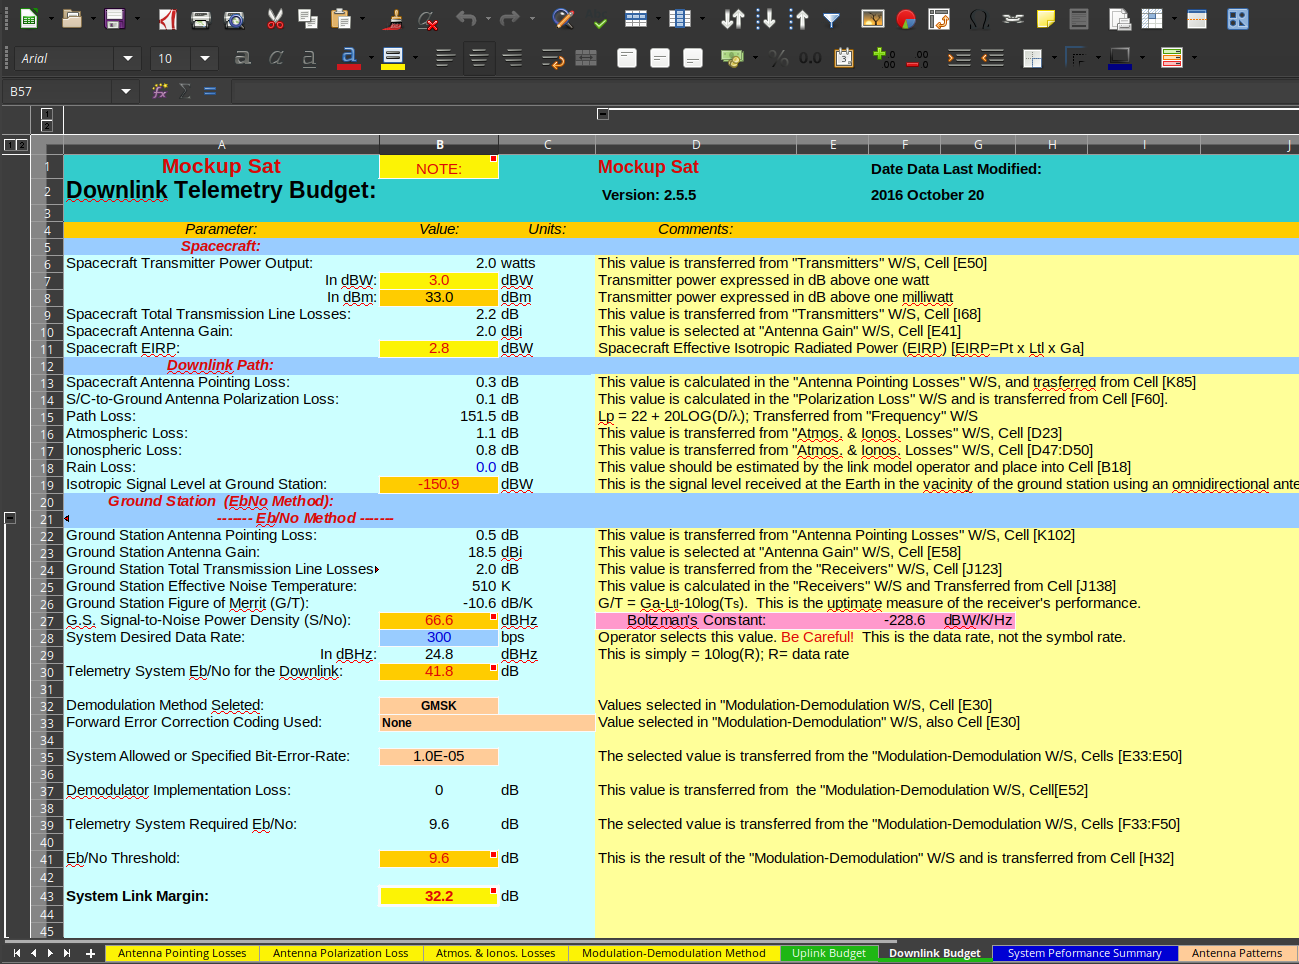
\includegraphics[width=\textwidth]{AMSAT.png}
				\caption{AMSAT.xls}
			\end{figure}
		\end{column}
		\hfill
		\begin{column}{.32\textwidth}
			\begin{figure}
				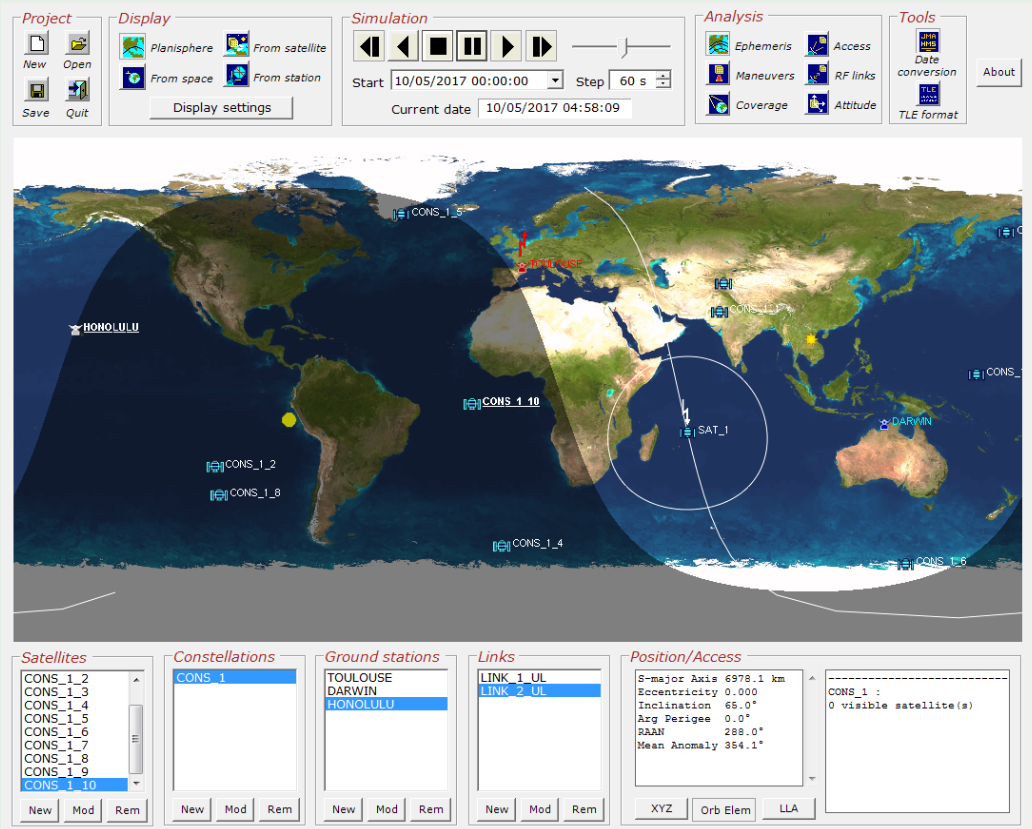
\includegraphics[width=\textwidth]{satorb.png}
				\caption{SatOrb}
			\end{figure}
		\end{column}
		\hfill
		\begin{column}{.32\textwidth}
			Python libraries : 
			\begin{itemize}
				\item linkpredict
				\item luplink
				\item ...
			\end{itemize}
		\end{column}
	\end{columns}
\end{frame}

\begin{frame}
	\frametitle{The Project : JSatOrb \& Luplink}
	%Open-source tool interfacing with NSS (inside JSatOrb)
	\begin{columns}[onlytextwidth]
		\begin{column}{.6\textwidth}
		\begin{figure}
			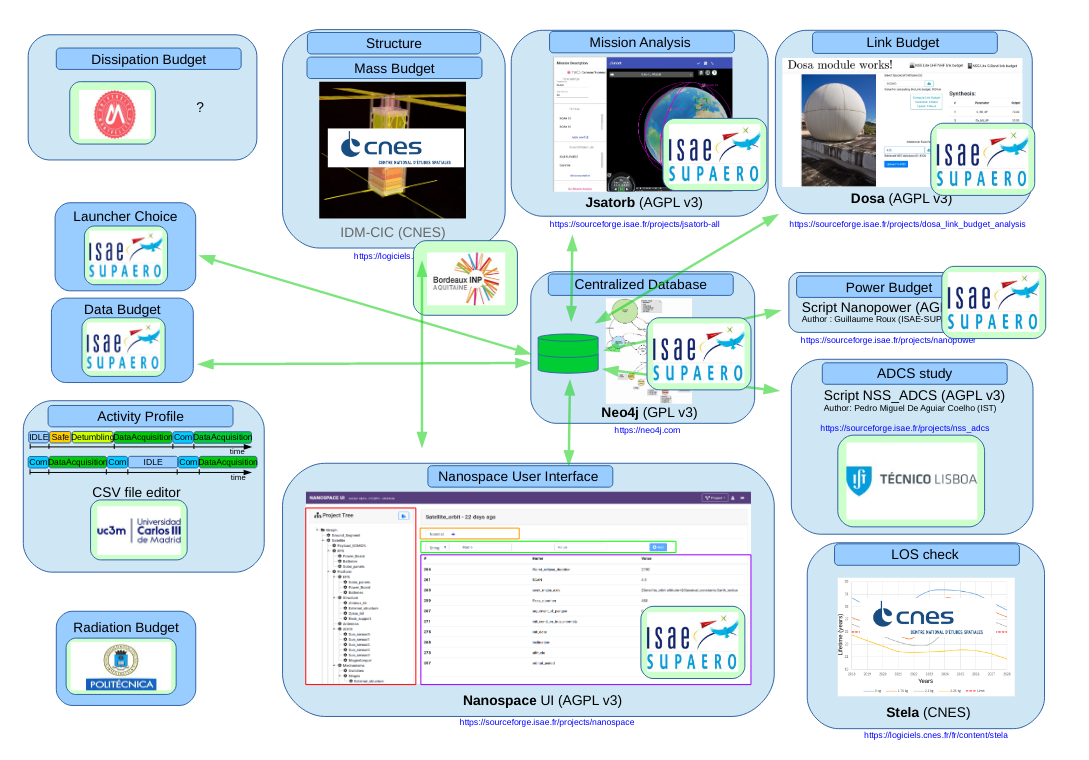
\includegraphics[width=\textwidth]{nss2.png}
			\caption{Nanospace Software Suite (NSS)}
		\end{figure}
	\end{column}
	\hfill
	\begin{column}{.35\textwidth}
	\alert{Luplink}: Open-source tool integrated inside JSatOrb.\\
	\bigskip
	
	Requirements : 
	\begin{itemize}
		\item Usable within NSS
		\item Suitable for teaching
		\item Modular
		\item Unit-tested
	\end{itemize}
	\end{column}
\end{columns}
%With web application frameworks, easy to build modular apps
\end{frame}

\begin{frame}
	\begin{figure}
		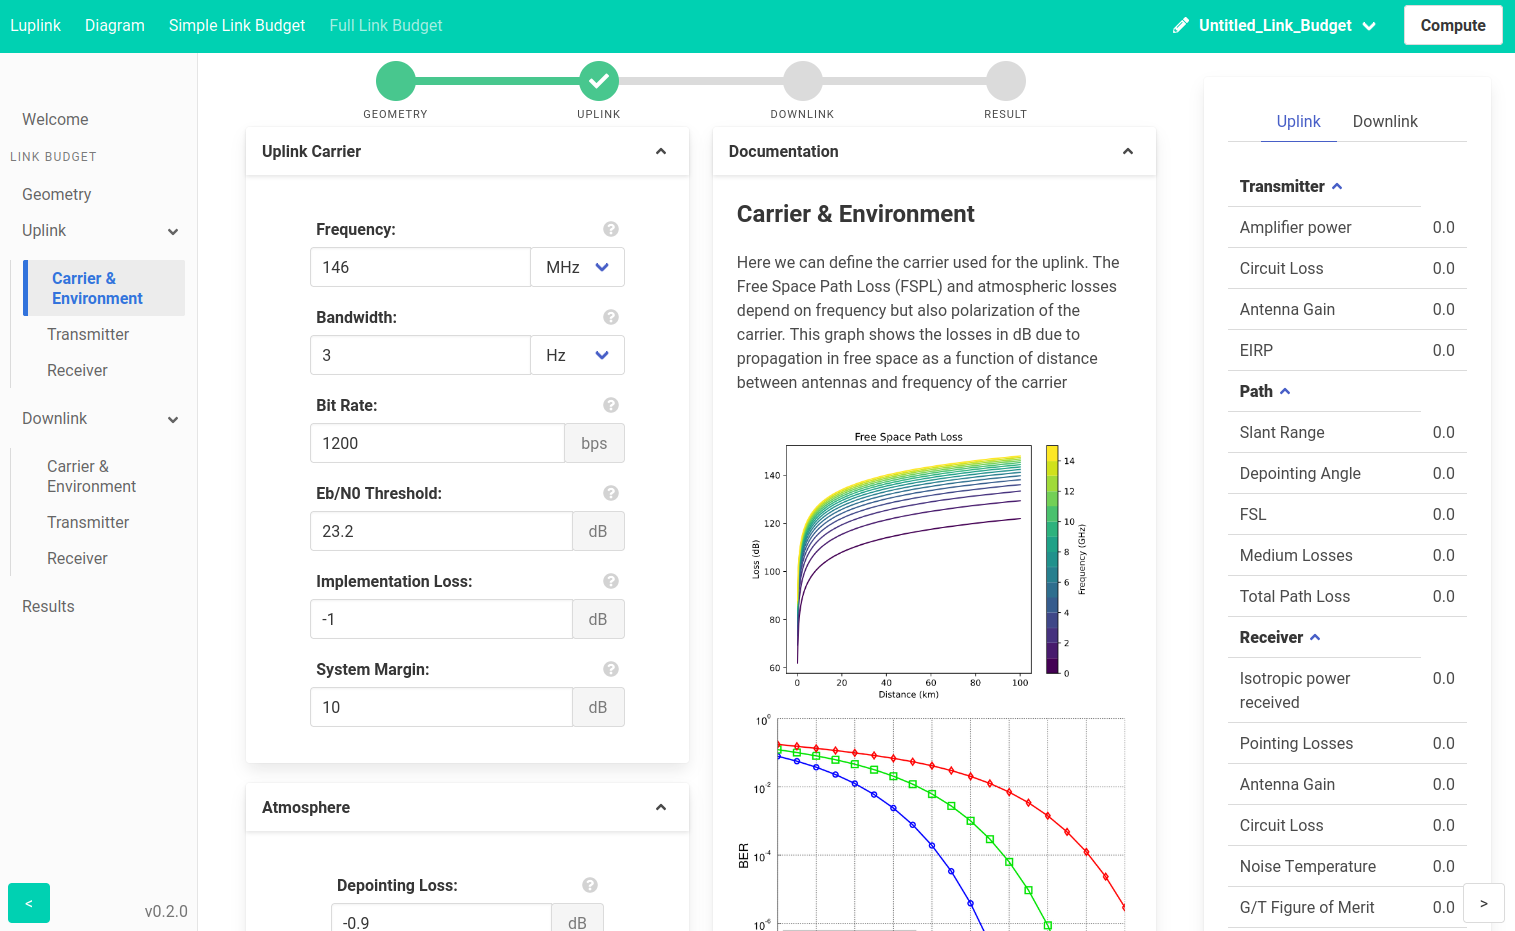
\includegraphics[width=\textwidth]{screenshot2.png}
			%\caption{Interface}
	\end{figure}
\end{frame}

\begin{frame}
	\begin{figure}
		\frametitle{Technologies used}
		\begin{columns}%
			\begin{column}{.4\textwidth}%
				\begin{itemize}
					\item Angular / TypeScript,
					\item Node.js
					\item SCSS/SASS,  
					\item Bulma,
					\item D3.js
					\item ...
				\end{itemize}
			\end{column}
			\begin{column}{.3\textwidth}
				\centering
					
\includegraphics[height=.15\textheight]{angular.png}
					
\includegraphics[height=.15\textheight]{typescript.png}
					
\includegraphics[height=.15\textheight]{sass.jpg}
					
\includegraphics[height=.15\textheight]{bulma.png}
					
\includegraphics[height=.15\textheight]{d3.jpeg}			
			\end{column}
		\end{columns}
	\end{figure}
\end{frame}
\begin{frame}
%	\begin{columns}
%		\begin{column}{.8\textwidth}%
			\begin{figure}
				\frametitle{Single Page Applications (SPA)}
				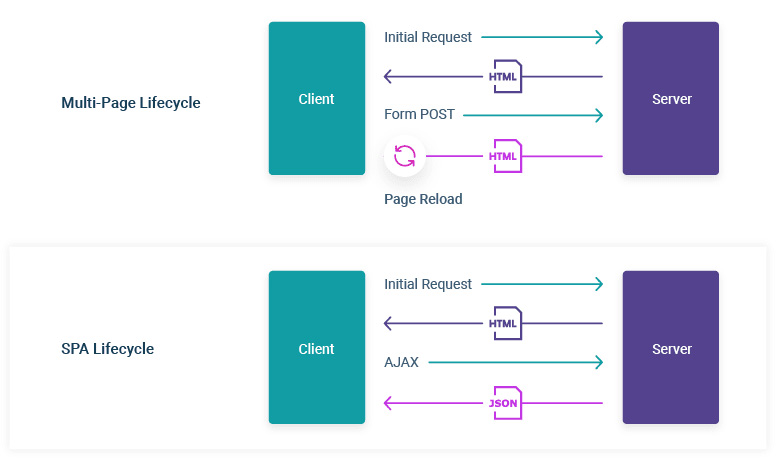
\includegraphics[width=.8\textwidth]{spa.jpg}
				%\caption{SPA vs Multi-Page Application (Credits: LVivity.com)}
			\end{figure}
%		\end{column}
\begin{columns}
		\begin{column}{1\textwidth}%
%			Advantages:
				\begin{itemize}
					
					\item No reload while navigating: faster load times
					\item Components are reusable
				\end{itemize}
	\end{column}
	\end{columns}
\end{frame}

\begin{frame}
\frametitle{Framework choice}
\begin{columns}[onlytextwidth]
	\begin{column}{0.6\textwidth}
		\begin{figure}
			
\includegraphics[width=0.4\textwidth]{angular.png}
			%\caption{Current UI}
		\end{figure}
		\bigbreak
Alternatives:
\bigbreak
\centering

\includegraphics[height=.15\textheight]{vuejs.png}

\includegraphics[height=.15\textheight]{react.png}
	\end{column}
	\hfill
	\begin{column}{0.45\textwidth}
		\textbf{Angular framework :} 
		\begin{itemize}
			\item Components,
			\item Typescript,  
			\item Good testing capabilities
			
			\item Used by JSatOrb (better integration)
		\end{itemize}
		
	\end{column}
\end{columns}

\end{frame}


\begin{frame}
	\frametitle{Project Architecture}
	\bigskip
	
	\begin{figure}
			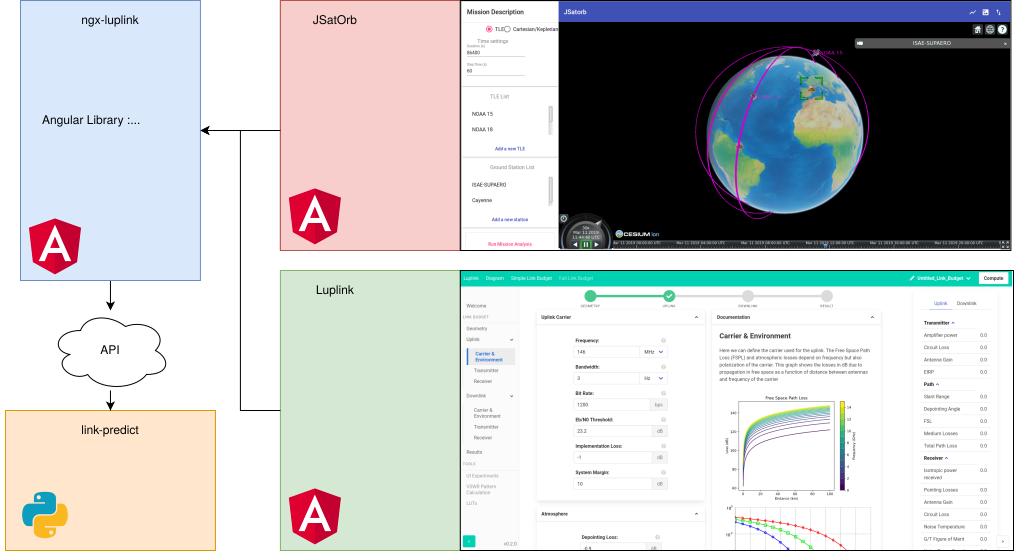
\includegraphics[width=\textwidth]{architecture1.png}
			%\caption{Current UI}
		\end{figure}
	\begin{columns}[onlytextwidth]
		
		\begin{column}{0.45\textwidth}
			
		\end{column}
		
		\begin{column}{0.6\textwidth}
	
		\end{column}
		
		\hfill
	\end{columns}
\end{frame}
%\begin{frame}
%	\frametitle{Project Architecture}
%	
%	\begin{columns}[onlytextwidth]
%		
%		\begin{column}{0.55\textwidth}
%			\begin{figure}
%			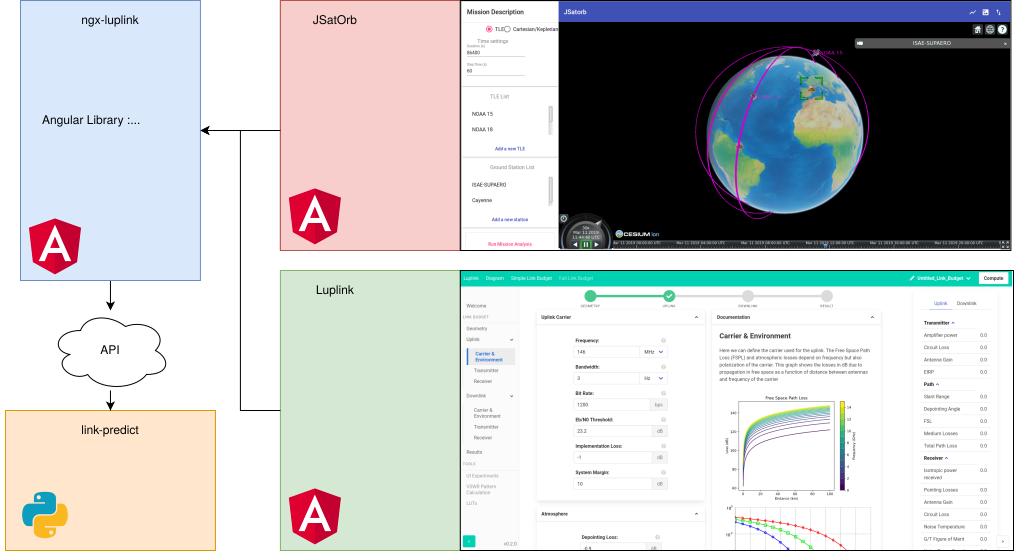
\includegraphics[width=\textwidth]{architecture1.png}
%			\caption{Current UI}
%		\end{figure}
%		\end{column}
%		
%		\begin{column}{0.6\textwidth}
%			\
%		\end{column}
%		
%		\hfill
%	\end{columns}
%\end{frame}
%\begin{frame}
%	\frametitle{Some challenges}
%	\begin{columns}[onlytextwidth]
%		\begin{column}{0.45\textwidth}
%			\begin{itemize}
%				\item Lots of inputs
%				\item Fit most use cases
%			\end{itemize}
%		\end{column}
%		
%		\begin{column}{0.6\textwidth}
%			\begin{figure}
%				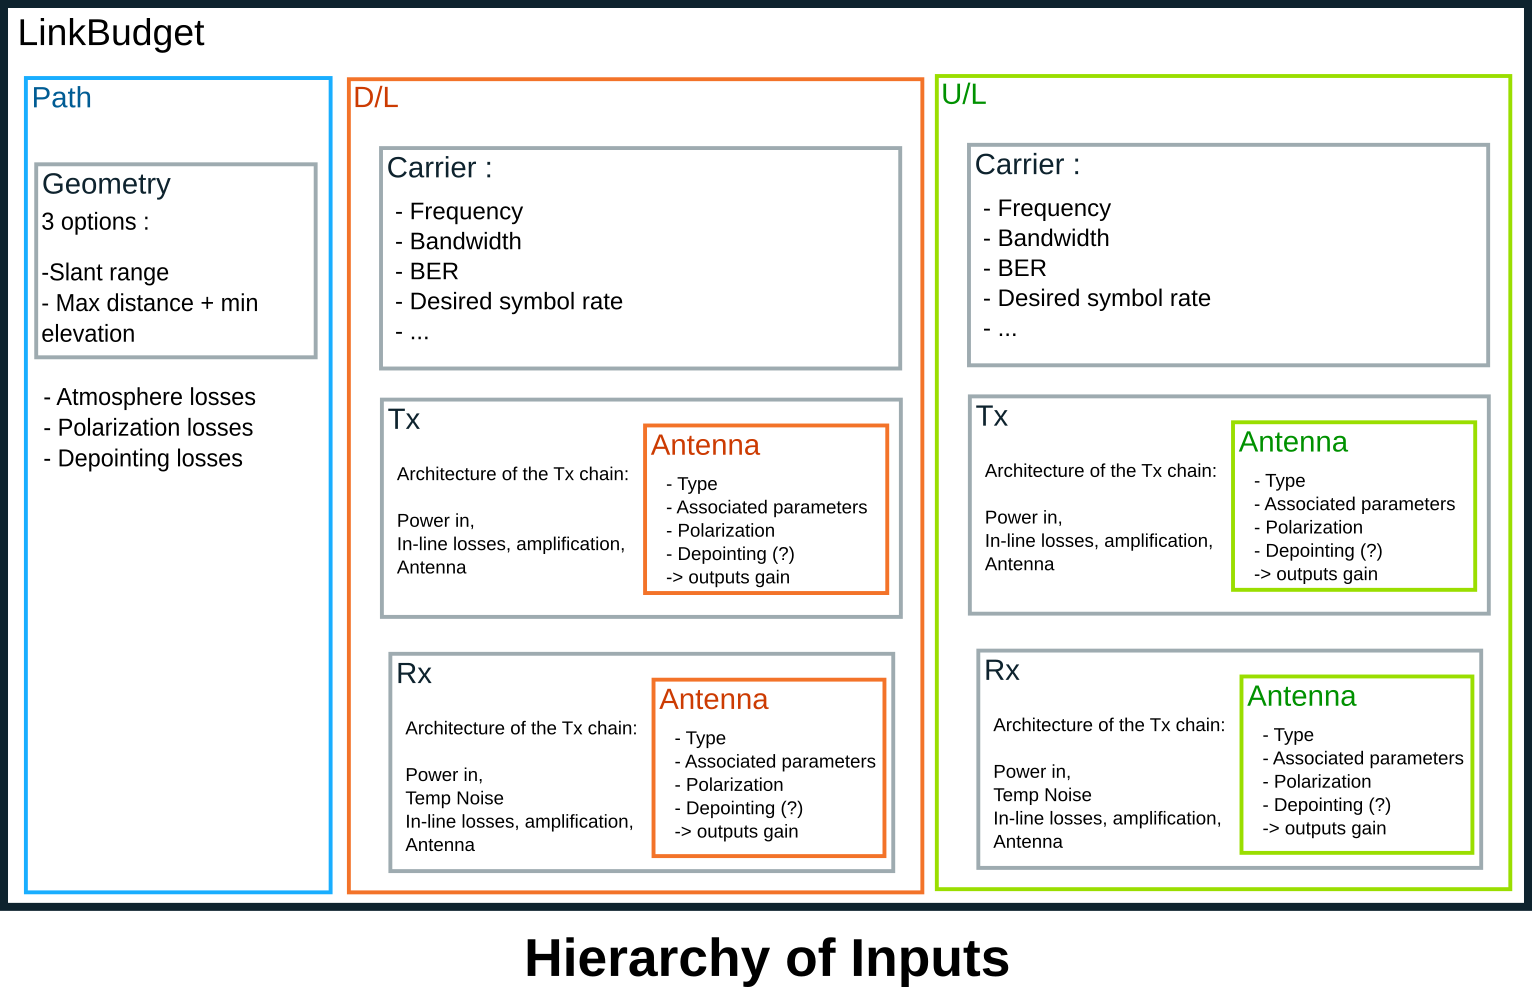
\includegraphics[width=\textwidth]{hierarchSimplified.png}
%				%\caption{Current UI}
%			\end{figure}
%		\end{column}
%		
%		\hfill
%	\end{columns}
%\end{frame}

%\begin{frame}
%\frametitle{Features}
%	\begin{columns}[onlytextwidth]
%		\begin{column}{0.5\textwidth}
%			\begin{itemize}
%				\item Computes static link-budget using linkpredict
%				\item Generate form from .json
%				\item Import files from JSatOrb
%				
%			\end{itemize}
%			\begin{figure}[hbtp]
%			\centering
%				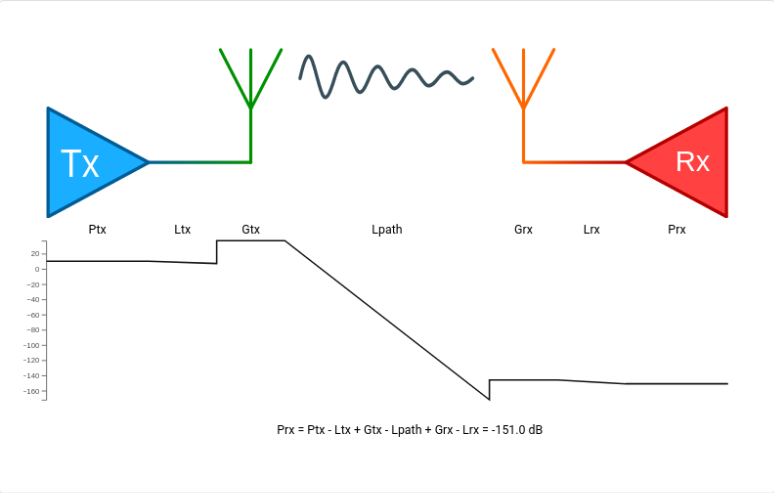
\includegraphics[width=\textwidth]{src/d3.png}
%				\caption{D3.js graph}
%			\end{figure}
%%			Next steps : 
%%			\begin{itemize}
%%			\item Full static link budget 
%%			\item Dynamic link budget
%		%Next :
%		%\end{itemize}
%		\end{column}
%		\hfill
%		\begin{column}{0.4\textwidth}
%			\begin{figure}[hbtp]
%				\centering
%				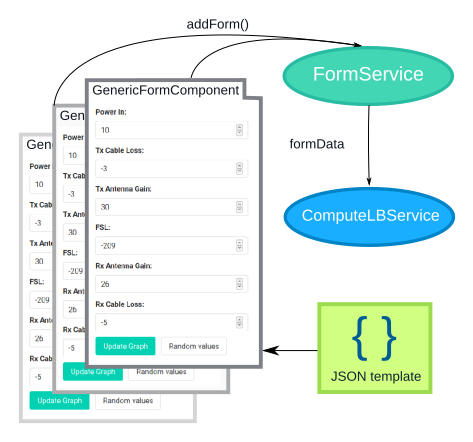
\includegraphics[width=\textwidth]{src/formArchSimplified.png}
%				\caption{Form Architecture}
%			\end{figure}
%			
%		\end{column}
%	\end{columns}
%	%UX issues : enough clarity while providing easy way to input data
%	%\textit{Difficulties : juggling with many options}
%	
%\end{frame}
\section{Usage}
\begin{frame}
	\begin{figure}
		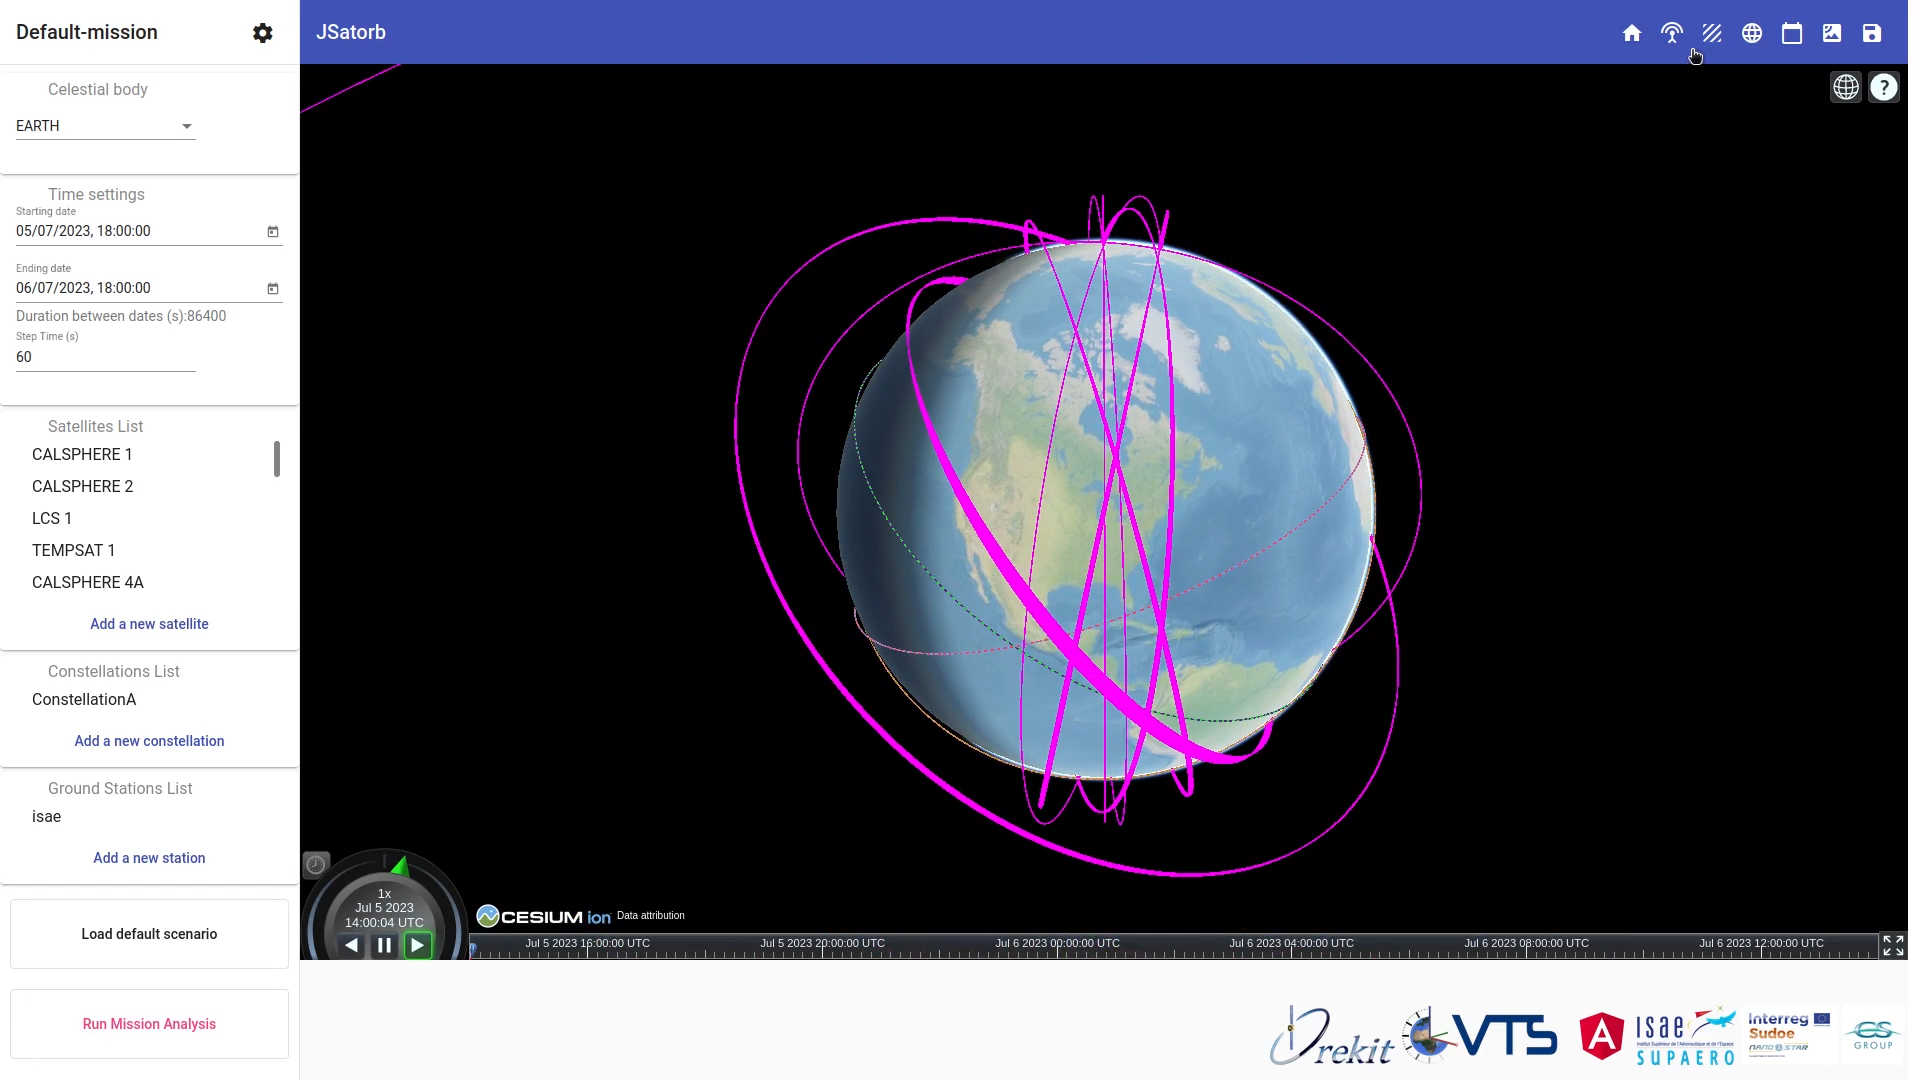
\includegraphics[width=1\textwidth]{1.png}
			%\caption{Interface}
	\end{figure}
\end{frame}
\begin{frame}
	\begin{figure}
		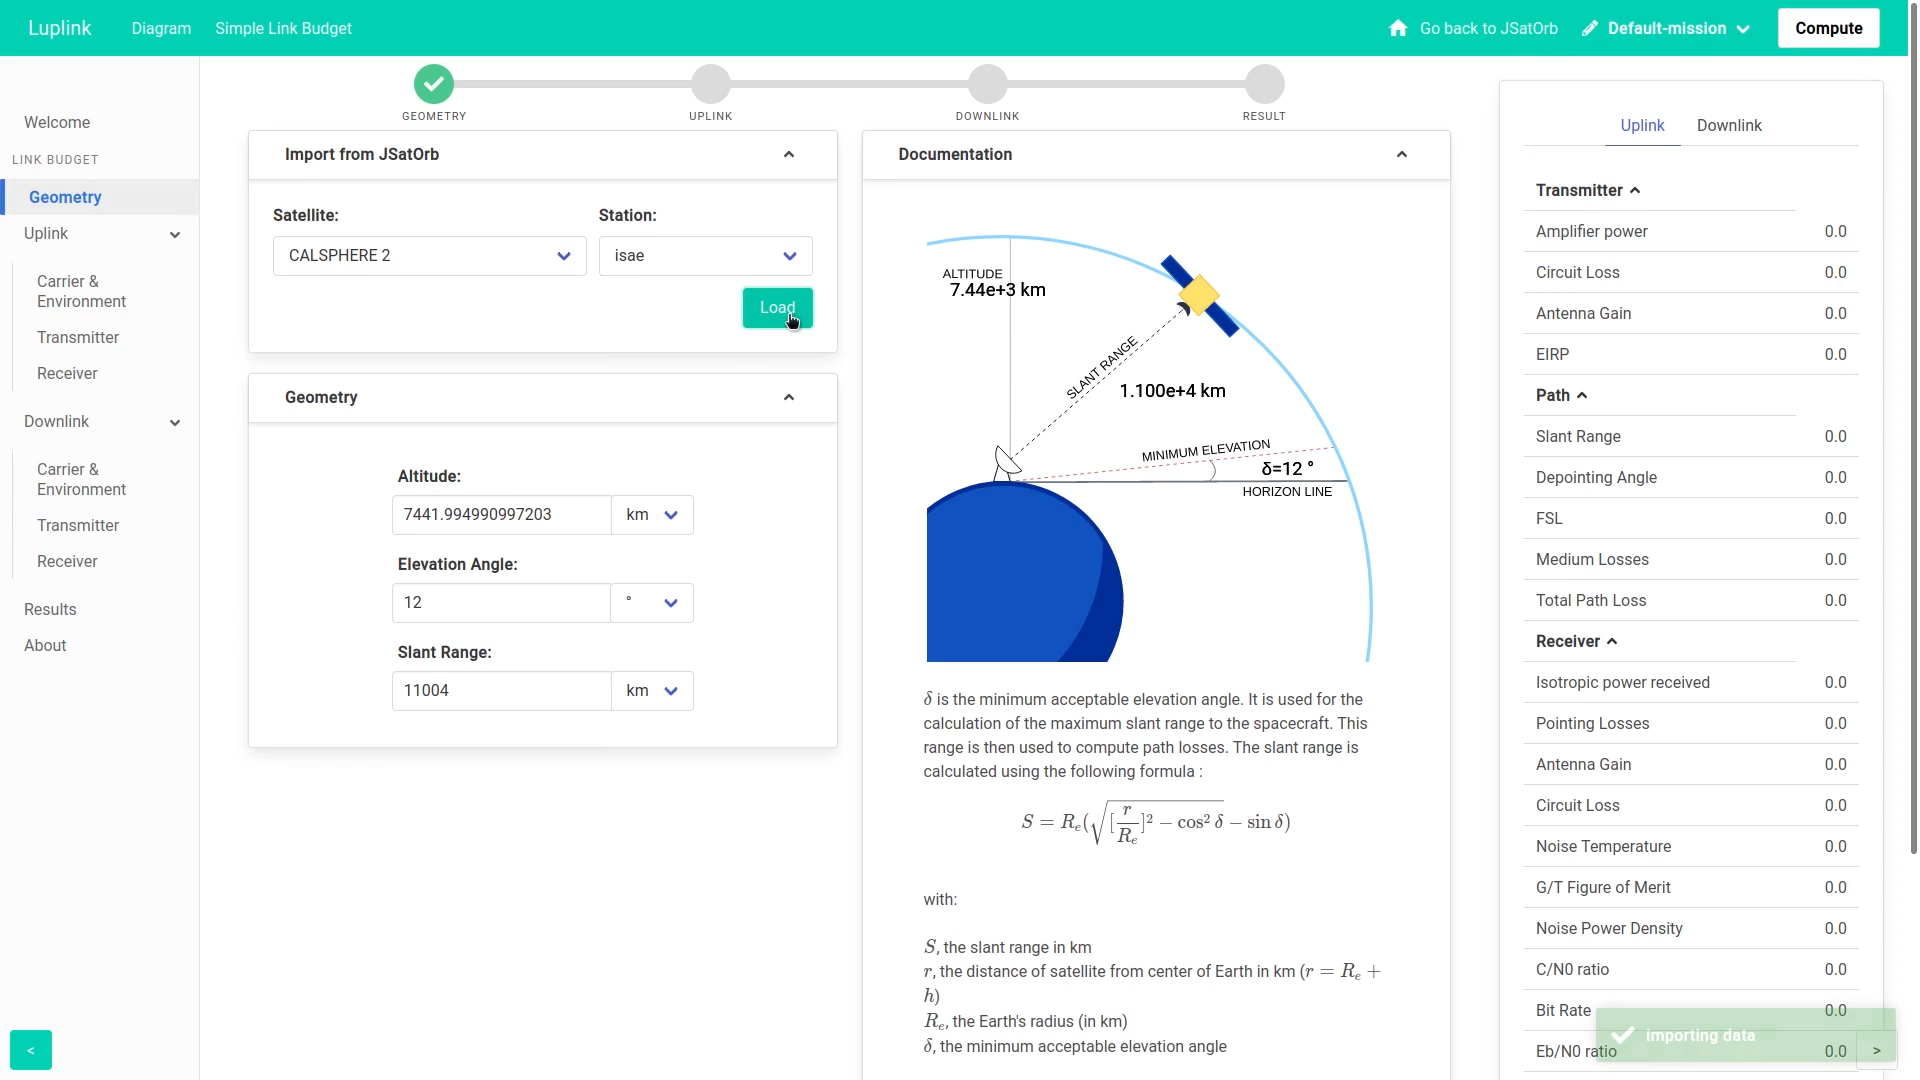
\includegraphics[width=1\textwidth]{2.png}
			%\caption{Interface}
	\end{figure}
\end{frame}
\begin{frame}
	\begin{figure}
		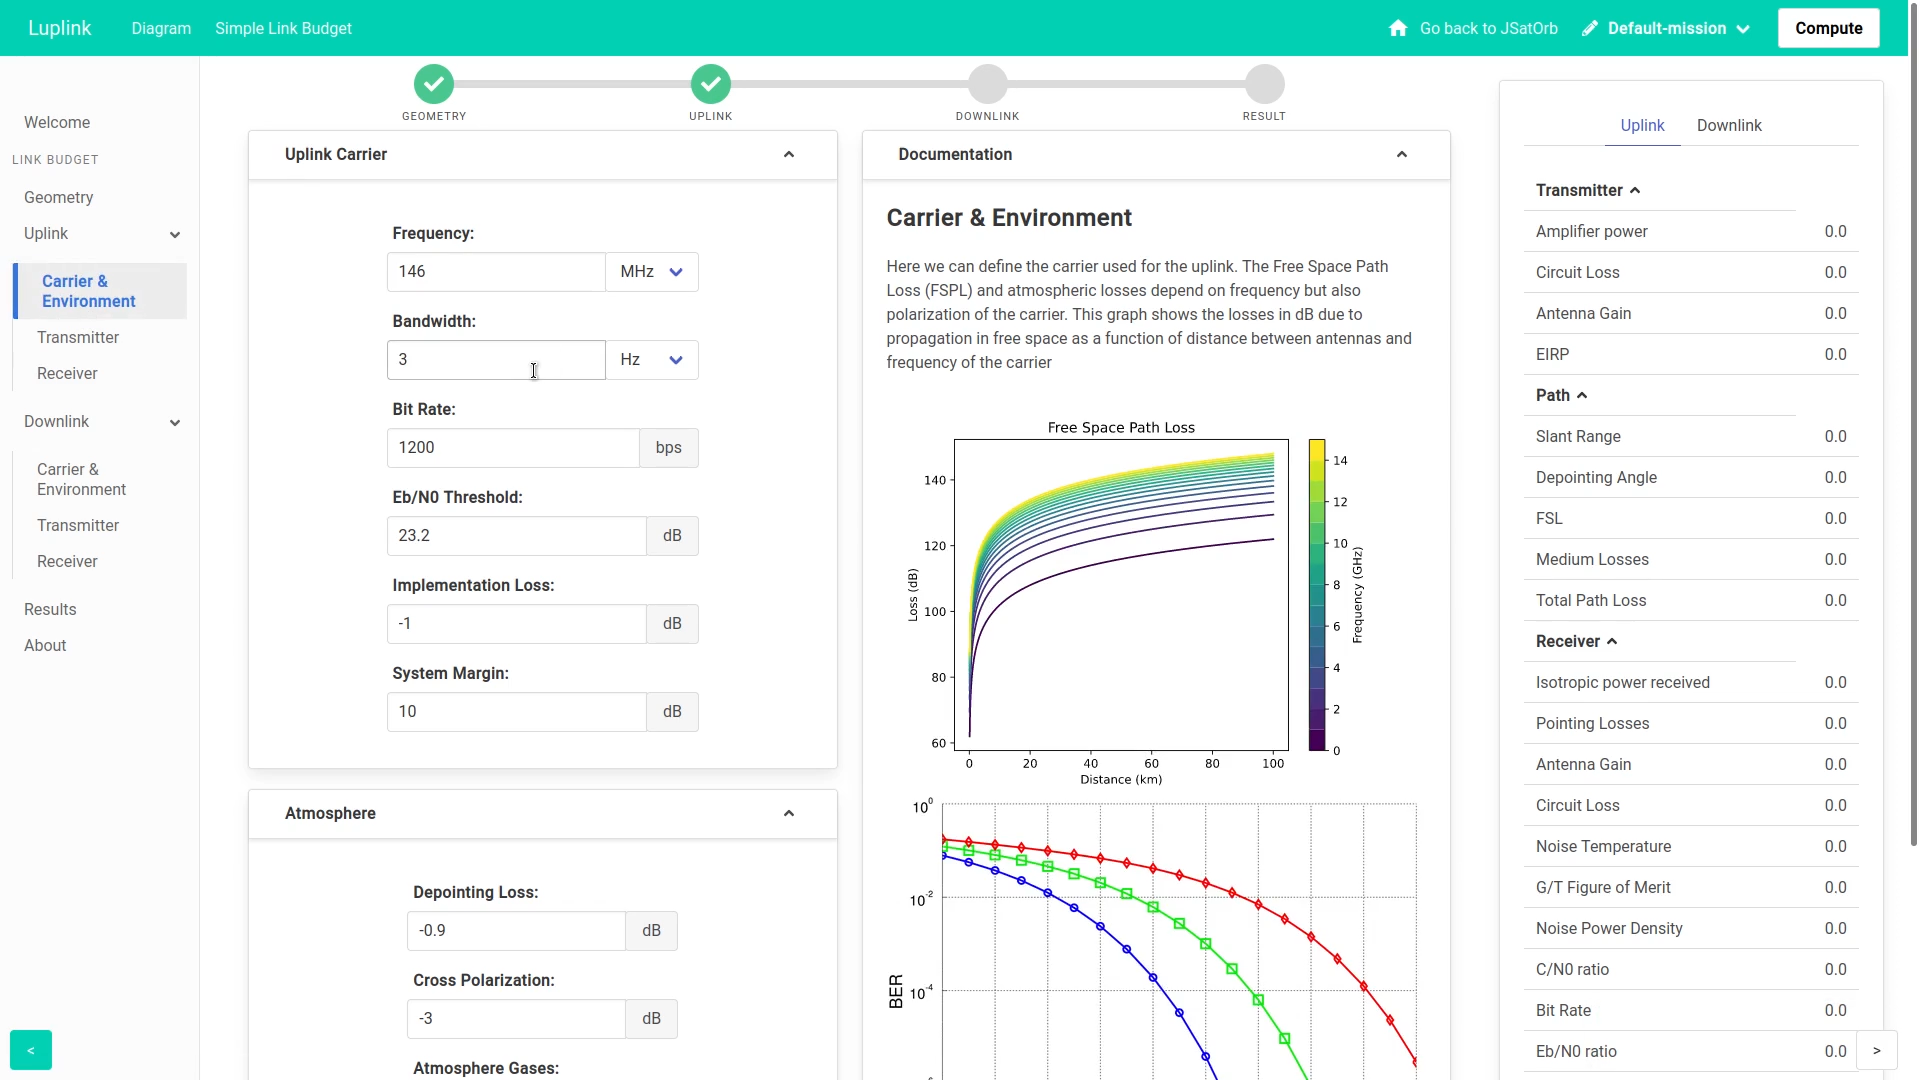
\includegraphics[width=1\textwidth]{3.png}
			%\caption{Interface}
	\end{figure}
\end{frame}
\begin{frame}
	\begin{figure}
		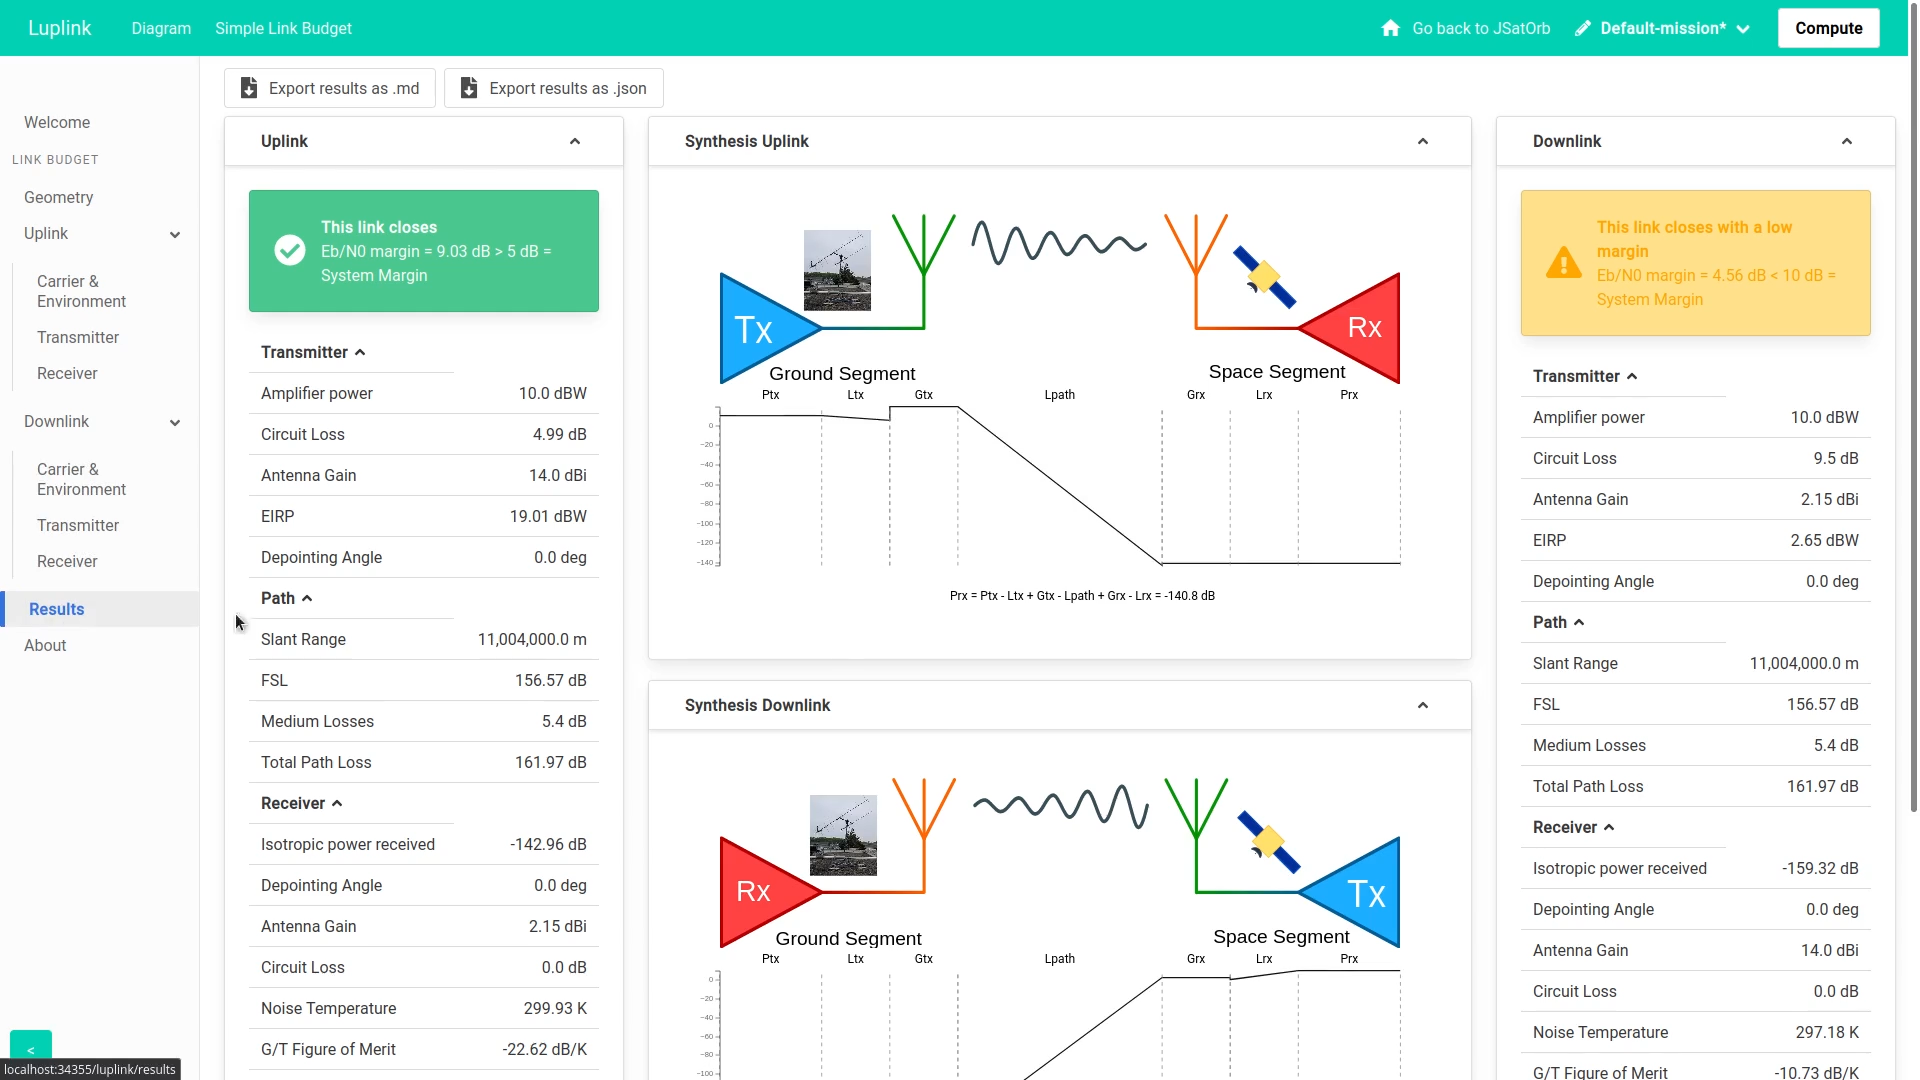
\includegraphics[width=1\textwidth]{4.png}
			%\caption{Interface}
	\end{figure}
\end{frame}
\begin{frame}
Thank you for your attention!
\end{frame}
\end{document}


